\subsection{Path loss: "Free space vs. building"}\label{sc:pathLoss}

To be able to understand the need for relaying, one must understand the boundaries of the chosen working environment. The range equation gives a good theoretical reference point to how a far a certain quality signal can be transmitted in optimal conditions. The range equation is dependent on transmission frequency and the characteristics of a transmitting and receiving antenna. The frequency dependency comes from the range equation calculation of the far field distance from the antenna pair. This far field distance occurs when the magnetic and electric part of the signal has a steady state phase relation. Also, the distance is dependent on the size and type of the antenna, while the telosb has a 2.7cm inverted f-antenna transmitting at a $2.408GHz$ center frequency. A $2.408GHz$ transmission frequency is chosen from the standard IEEE\_802.15.4, making $2.401GHz$ a "1" and $2.408$ a "0". Trying to keep the frequency as low as possible gives longer transmission ranges both in theory and in practice, as the lower frequencies have better penetration chances given obstacles. The radiation pattern, $-3dB$ power line, of a Ferrite-based inverted F-antenna can be seen in figure \ref{fig:invertedAntenna} [6]. Focusing on protocol and power consumption, the range equation will be visualized based on an omnidirectional antenna with same polarization, that is isotropic.

\noindent The telosb software specifies transmission power in dBm and the receiving/transmitting antenna have same the characteristics, so the need to understand the antennas workings beyond the far field distance estimation is not needed for this project. Since our main focus is a packet control protocol, each antenna is treated as isotropic being able to broadcast up to $100m$ in each direction as specified in the data sheet of the CC2420\footnote{\cite{Ieee}}. To simulate a real scenario, the transmitting antenna could be mounted on a rotational motor following the runner using computer vision hence the main beam, e.g. $153\deg$, of the antenna pattern would always point towards the runner verifying our calculation approach. Giving a far field distance of $0.01167m$ and optimal conditions in air, figure \ref{fig:logpathReceivedSignal_baseStation_air_highSignal} shows the expected received signal strength indication in dBm based on the range equation \ref{eq:rangeEquation} and the assumed assumptions.

\begin{figure}[h]
	\centering
	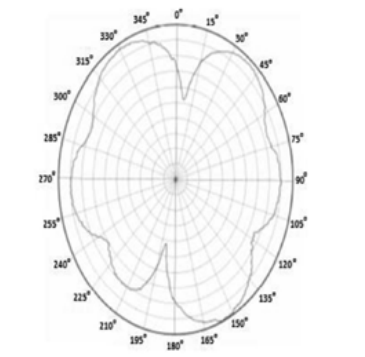
\includegraphics[width=1\linewidth]{theory/pathLoss/fig/invertedAntenna.png}
	\caption{Estimation of an inverted-F antenna's radiation pattern.}
	\label{fig:invertedAntenna}
\end{figure}

\begin{figure}[h]
	\begin{flalign*}
		f &= 2.407 \cdot 10^{9} Hz \qquad
		D = 2.7 \cdot 10^{-3} m \\
		\lambda &= \frac{c}{f} = 0.125m \qquad
		\gamma_{air} = 2 \qquad
		\gamma_{building} = 5.5\\
		d{0} &= \frac{2 \cdot D^{2}}{\lambda} = 1.171 \cdot 10^{-4} m
	\end{flalign*}
	
	\begin{subequations}
		\begin{align}
			P_{rcvd}(d) &= \frac{ P_{tx} \cdot G_{t} \cdot G_{r} \cdot \lambda^{2} }{ (4 \pi)^{2} \cdot d^{2} \cdot L }\\
			&= \frac{ P_{tx} \cdot G_{t} \cdot G_{r} \cdot \lambda^{2} }{ (4 \pi)^{2} \cdot d_{0}^{2} \cdot L } \cdot \bigg (\frac{d_{0}}{d} \bigg )^{2}\\
			&= P_{rcvd}(d_{0}) \cdot \bigg (\frac{d_{0}}{d} \bigg )^{\gamma}
		\end{align}
	\end{subequations}
	\caption{Range equation based on a $2.7cm$ wide inverted f-antenna and a $2.408GHz$ center frequency}
	\label{eq:rangeEquation}
\end{figure}

%Figure 3
\begin{figure}[h]
	\centering
	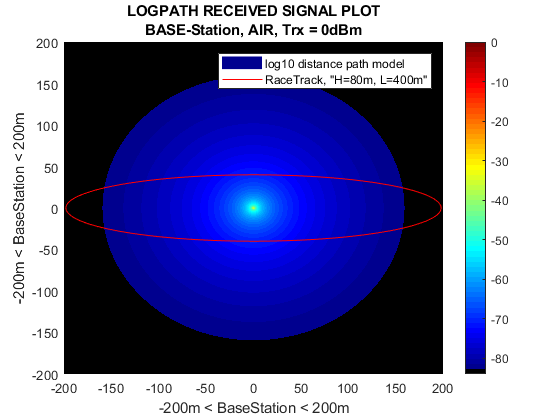
\includegraphics[width=1\linewidth]{theory/pathLoss/fig/logpathReceivedSignal_baseStation_air_highSignal.png}
	\caption{$-84dBm$ $159.3m$ received signal area of the running track. The antenna cannot cover the entire track.}
	\label{fig:logpathReceivedSignal_baseStation_air_highSignal}
\end{figure}

\noindent Given a racetrack of $400m$ in width, under optimal conditions as shown in figure \ref{fig:logpathReceivedSignal_baseStation_air_highSignal} a telosb node will not be able to cover the entire track and two additional relay "hop" stations must be installed to provide sufficient cover. The antenna dimensions and transmission power gives a natural boundary to which relaying will be the only option. Figure \ref{fig:logpathReceivedSignal_eachStation_air_highSignal} shows the RF input power of two relay stations in comparison to the base station, while figure 4 \ref{fig:logpathReceivedSignal_combinedStations_air_highSignal} shows the combined RF input power of the runner node.

%Figure 4
\begin{figure}[h]
	\centering
	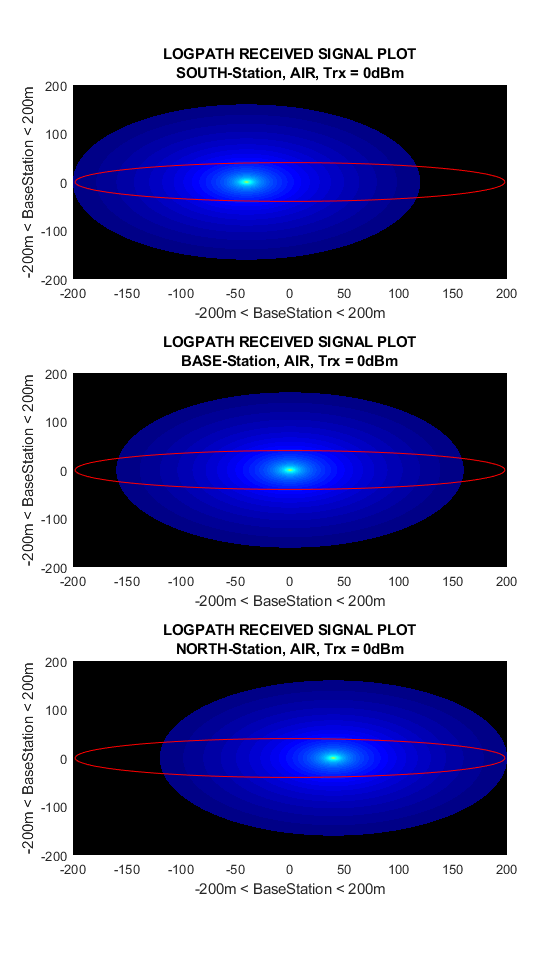
\includegraphics[width=1\linewidth]{theory/pathLoss/fig/logpathReceivedSignal_eachStation_air_highSignal.png}
	\caption{Three stations covering the entire track individually.}
	\label{fig:logpathReceivedSignal_eachStation_air_highSignal}
\end{figure}

\begin{figure}[h]
	\centering
	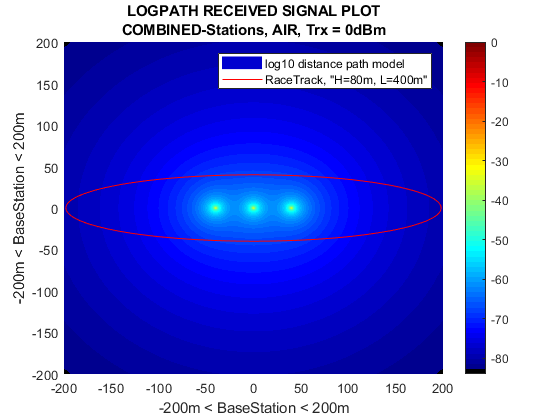
\includegraphics[width=1\linewidth]{theory/pathLoss/fig/logpathReceivedSignal_combinedStations_air_highSignal.png}
	\caption{Three stations covering the entire track combined.}
	\label{fig:logpathReceivedSignal_combinedStations_air_highSignal}
\end{figure}

\noindent Lowering the transmission power can prolong the lifetime of individual nodes and the wireless network all together, but at the cost of less coverage. Figure \ref{fig:logpathReceivedSignal_baseStation_air_lowSignal} shows the single and \ref{fig:logpathReceivedSignal_combinedStations_air_lowSignal} the combined RF input power of the runner node with all nodes using transmission power of $-24dBm$. The size of the track is now only $7.5\%$ of the full power track. 

%Figure 5
\begin{figure}[h]
	\centering
	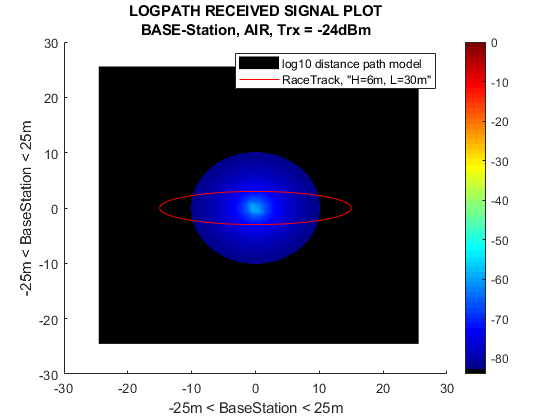
\includegraphics[width=1\linewidth]{theory/pathLoss/fig/logpathReceivedSignal_baseStation_air_lowSignal.png}
	\caption{$10.1m$ adequate RF input power for the base station.}
	\label{fig:logpathReceivedSignal_baseStation_air_lowSignal}
\end{figure}

\begin{figure}[h]
	\centering
	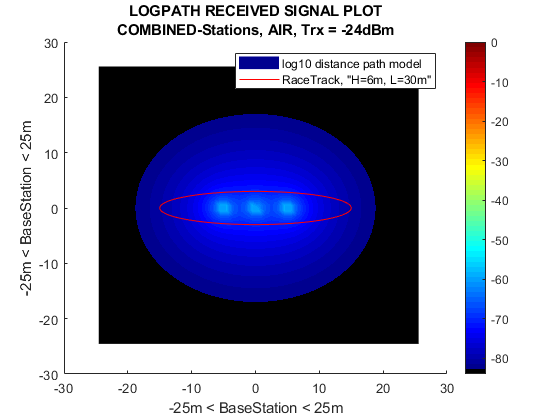
\includegraphics[width=1\linewidth]{theory/pathLoss/fig/logpathReceivedSignal_combinedStations_air_lowSignal.png}
	\caption{$10.1m$ Three stations combined RF input power.}
	\label{fig:logpathReceivedSignal_combinedStations_air_lowSignal}
\end{figure}

\noindent Further reduction in RF input power can happen for multiple reasons, e.g: reflection, diffraction, scattering and Doppler fading. An easy noise model can be to change $\gamma_{air}$ in equation \ref{eq:rangeEquation} to $\gamma_{building}$ with values taken from page 93 [REF 1]. Figure \ref{fig:logpathReceivedSignal_baseStation_office_lowSignal} and \ref{fig:logpathReceivedSignal_combinedStations_office_lowSignal} show the distance at minimum transmitted power (PTX) inside a building providing a stunning $0.035\%$ of the coverage related to full power in open AIR.

\begin{figure}[h]
	\centering
	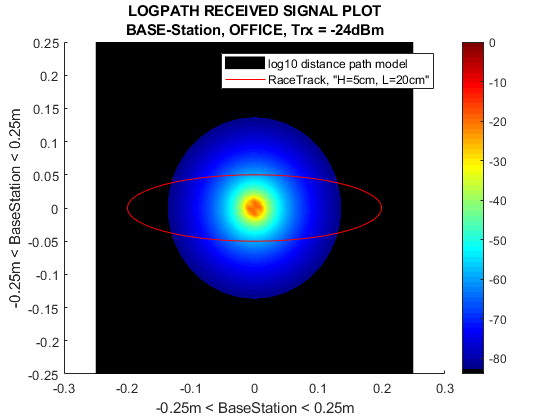
\includegraphics[width=1\linewidth]{theory/pathLoss/fig/logpathReceivedSignal_baseStation_office_lowSignal.png}
	\caption{$13.1cm$ adequate RF input power for the base station.}
	\label{fig:logpathReceivedSignal_baseStation_office_lowSignal}
\end{figure}

\begin{figure}[h]
	\centering
	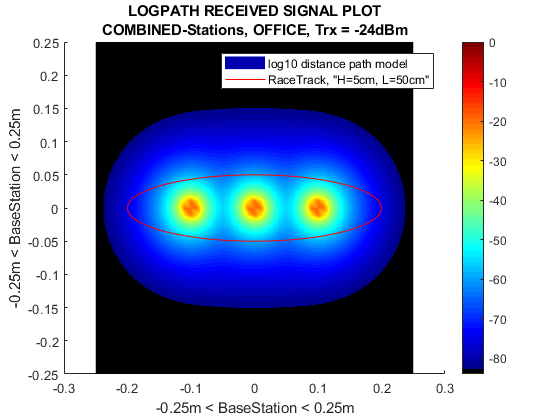
\includegraphics[width=1\linewidth]{theory/pathLoss/fig/logpathReceivedSignal_combinedStations_office_lowSignal.png}
	\caption{$13.1cm$ Three stations combined RF input power.}
	\label{fig:logpathReceivedSignal_combinedStations_office_lowSignal}
\end{figure}